\documentclass[conference]{IEEEtran}
\IEEEoverridecommandlockouts
\usepackage{cite}
\usepackage{amsmath,amssymb,amsfonts}
\usepackage{graphicx}
\usepackage{textcomp}
\usepackage{xcolor}
\usepackage{hyperref}
\hypersetup{hidelinks}
\usepackage{array}
\usepackage{xurl}

\hypersetup{
    breaklinks=true,
    colorlinks=false
}

\def\BibTeX{{\rm B\kern-.05em{\sc i\kern-.025em b}\kern-.08em
    T\kern-.1667em\lower.7ex\hbox{E}\kern-.125emX}}

\begin{document}
\bstctlcite{IEEEexample:BSTcontrol}
\title{% TODO: Título definitivo del proyecto.
Detección de Inundaciones Urbanas en Lima Sur mediante Imágenes SAR Sentinel-1 y Redes Neuronales Convolucionales\\
}

% TODO: completar autores, afiliación y correos de cada integrante.
\author{
\IEEEauthorblockN{1\textsuperscript{st} Yoel Miranda}
\IEEEauthorblockA{\textit{Facultad de Ingeniería} \\
\textit{Universidad ESAN}\\
Lima, Perú \\
24200215@ue.edu.pe}
\and
\IEEEauthorblockN{2\textsuperscript{nd} Andrés Quiliche}
\IEEEauthorblockA{\textit{Facultad de Ingeniería} \\
\textit{Universidad ESAN}\\
Lima, Perú \\
22200144@ue.edu.pe}
\and
\IEEEauthorblockN{3\textsuperscript{rd} Jummy Gave}
\IEEEauthorblockA{\textit{Facultad de Ingeniería} \\
\textit{Universidad ESAN}\\
Lima, Perú \\
22200224@ue.edu.pe}
\and
\IEEEauthorblockN{4\textsuperscript{th} Jefferson Garay}
\IEEEauthorblockA{\textit{Facultad de Ingeniería} \\
\textit{Universidad ESAN}\\
Lima, Perú \\
22200217@ue.edu.pe}

}


\maketitle

% ============================================================
% RESUMEN / ABSTRACT
% TODO: 150-200 palabras. Problema, método, dato, y qué se espera
% demostrar. Se escribe al final, cuando ya está clara la
% introducción y el estado del arte.
% ============================================================

% ============================================================
% I. INTRODUCCIÓN
% ============================================================
\section{Introducción}
\label{sec:introduccion}

Las inundaciones urbanas constituyen un problema relevante para la gestión del riesgo de desastres debido a sus posibles efectos sobre viviendas, vías de comunicación, infraestructura pública y servicios básicos. En Lima Sur, distritos como Villa María del Triunfo y Villa El Salvador han sido considerados en acciones de prevención frente a episodios de lluvias intensas. En marzo de 2023, Villa El Salvador fue declarado en estado de emergencia por peligro inminente ante precipitaciones pluviales \cite{vesEmergencia2023}, mientras que la municipalidad distrital realizó recorridos preventivos en sus zonas más vulnerables \cite{vesLluvias2023}. Asimismo, en Villa María del Triunfo se activó el Centro de Operaciones de Emergencia Distrital (COED) y se realizaron acciones de supervisión de drenajes y caídas de quebradas en zonas consideradas de alto riesgo ante lluvias prolongadas \cite{vmtLluvias2023}. A diferencia de una inundación fluvial típica, asociada al desborde de un río, en sectores urbanos de Lima Sur el problema puede manifestarse mediante anegamientos, escorrentía superficial y acumulación de agua en vías y zonas de pendiente.

El monitoreo de estos eventos presenta dificultades debido a que la información disponible puede provenir de inspecciones en campo, reportes municipales y registros institucionales generados durante la emergencia. Aunque estas fuentes son necesarias para las acciones de prevención y respuesta, resulta pertinente complementarlas con herramientas que permitan analizar de manera espacial y sistemática la presencia de agua y delimitar las zonas potencialmente afectadas.

En este contexto, las imágenes de Radar de Apertura Sintética (SAR) de la misión Sentinel-1 representan una alternativa adecuada para el monitoreo de inundaciones. Al tratarse de un sensor activo de microondas, Sentinel-1 puede adquirir información tanto de día como de noche y bajo condiciones de nubosidad \cite{copernicusSentinel1}. Además, las superficies cubiertas por agua presentan patrones particulares de retrodispersión que permiten analizar cambios respecto de otras coberturas y apoyar la identificación de zonas con presencia de agua \cite{bonafilia2020sen1floods11}.

Sin embargo, persisten limitaciones importantes en los enfoques existentes. Kuro Siwo demuestra la utilidad de las series temporales SAR para el mapeo de inundaciones, pero sus etiquetas de referencia fueron elaboradas manualmente por especialistas, lo que demanda tiempo y recursos \cite{bountos2024kurosiwo}. Por otro lado, Sen1Floods11 constituye un dataset de referencia para la detección de inundaciones mediante Sentinel-1, mientras que UrbanSARFloods evidencia que la detección en entornos urbanos representa un reto adicional debido a la interacción de la señal radar con edificaciones y otras estructuras \cite{bonafilia2020sen1floods11,zhao2024urbansarfloods}. En un contexto como Lima Sur, donde la disponibilidad de máscaras locales de inundación es limitada, la generación automática de etiquetas mediante técnicas de detección de cambio constituye una alternativa para reducir la dependencia de anotaciones manuales. Este enfoque encuentra respaldo en trabajos como Sen1Floods11 y en el método no supervisado propuesto por Yadav et al., que demuestra la utilidad de series temporales SAR para detectar cambios asociados a inundaciones \cite{bonafilia2020sen1floods11,yadav2024unsupervised}.

Por ello, el objetivo del presente trabajo es desarrollar y evaluar un modelo de segmentación basado en redes neuronales convolucionales para detectar y delimitar zonas con presencia de agua en imágenes SAR Sentinel-1, con aplicación en Lima Sur. El entrenamiento y la validación se realizarán con datasets internacionales de referencia, mientras que las imágenes correspondientes a Lima se emplearán para la prueba y aplicación del modelo. El resto del documento se organiza de la siguiente manera:
la Sección~\ref{sec:estado-del-arte} presenta los antecedentes;
la Sección~\ref{sec:metodologia} describe la metodología
propuesta, incluyendo los conjuntos de datos, su preparación,
el entrenamiento y la evaluación; y las secciones posteriores
presentarán los experimentos, resultados y conclusiones.

% --- Párrafo 1: el problema, con datos duros ---
% TODO: contextualizar las inundaciones recientes en Villa María del
% Triunfo y Villa El Salvador. Mencionar fechas de eventos, cifras de
% afectados si se consiguen (prensa, INDECI/COEN), y por qué el
% anegamiento urbano en Lima Sur es distinto de la inundación fluvial
% típica (topografía de ladera, drenaje insuficiente, asentamiento
% informal).

% --- Párrafo 2: por qué el monitoreo actual es insuficiente ---
% TODO: explicar que hoy no existe un sistema automatizado que mapee
% la extensión de una inundación en estas zonas; el mapeo, cuando
% ocurre, depende de inspección manual o reportes dispersos.

% --- Párrafo 3: la oportunidad técnica (SAR) ---
% TODO: explicar en 2-3 líneas por qué SAR es la herramienta correcta
% (atraviesa nubes, funciona de noche, el agua tiene una firma de
% retorno de radar muy distinta a la tierra).

% --- Párrafo 4: el vacío que atacan (gap) ---
% TODO: explicar que los modelos existentes dependen de etiquetas manuales
% costosas (Kuro Siwo) y que se han enfocado en inundaciones de áreas
% abiertas, no urbanas (UrbanSARFloods, Sen1Floods11). Lima Sur es
% inundación urbana en un contexto con escasez de datos. Por ello, la
% propuesta genera etiquetas automáticas por detección de cambio, enfoque
% respaldado por Sen1Floods11 y Yadav et al. (ver Sección II-E).

% --- Párrafo 5: objetivo y estructura del documento ---
% TODO: una frase de objetivo general, y un cierre tipo "el resto del
% documento se organiza como sigue: la Sección II revisa el estado
% del arte, la Sección III describe la metodología propuesta, [...]".

% ============================================================
% II. ESTADO DEL ARTE
% Mínimo 4 antecedentes. Cada uno con: Título/autores/año, Problema,
% BD, Técnicas, Metodología, Resultados.
% Se recomienda una subsección por antecedente para que sea fácil de
% leer y de completar en paralelo por distintos integrantes.
% ============================================================
\section{Estado del Arte}
\label{sec:estado-del-arte}

En esta sección se revisan cinco trabajos que sustentan la propuesta. Tres de ellos son conjuntos de datos de referencia para el mapeo de inundaciones con imágenes de radar Sentinel-1 (Kuro Siwo, UrbanSARFloods y Sen1Floods11); uno propone un método de detección de cambio que no requiere etiquetas (Yadav et al.); y el quinto es una solución de segmentación basada en conjuntos de U-Net para la competencia ETCI 2021 (Paul y Ganju). Para cada antecedente se describe el problema abordado, la base de datos, las técnicas, la metodología y los resultados.

% ------------------------------------------------------------
\subsection{Kuro Siwo: A Global Multi-Temporal Satellite Dataset for Rapid Flood Mapping \cite{bountos2024kurosiwo}}

\textbf{Autores y año:} N.~I. Bountos, M. Sdraka, A. Zavras, I. Karasante, A. Karavias, T. Herekakis, A. Thanasou, D. Michail e I. Papoutsis (2024). Publicado en NeurIPS 2024, Datasets and Benchmarks Track.

\textbf{Problema:} El radar de apertura sintética (SAR) permite observar la superficie de día y de noche y bajo cualquier condición climática; sin embargo, su uso en aprendizaje profundo para segmentar inundaciones está limitado por la falta de datasets grandes y bien anotados. Los autores identifican dos causas: el ruido \textit{speckle} propio del SAR y la escasez de datos de entrenamiento curados. Más aún, señalan que muchos datasets previos incluyen solo la imagen posterior al evento y omiten la imagen previa, que es justamente la que permite distinguir el agua permanente de la inundación.

\textbf{Base de datos:} Kuro Siwo reúne 43 eventos de inundación ocurridos entre 2015 y 2022 en seis continentes y tres zonas climáticas. Para cada evento se conforma un triplete Sentinel-1 a 10~m de resolución: dos imágenes previas y una posterior, en polarizaciones VV y VH, en formato GRD y SLC. El componente etiquetado contiene 67\,490 series temporales (202\,470 muestras SAR) en teselas de $224\times224$ píxeles, acompañadas de un modelo de elevación SRTM. Las etiquetas fueron producidas manualmente por un equipo de cinco expertos en SAR en tres clases: sin agua, agua permanente e inundación. Además, el dataset incluye un componente sin etiquetar de 533\,847 series temporales (1\,601\,511 muestras) para aprendizaje autosupervisado.

\textbf{Técnicas:} Los autores proponen el benchmark BlackBench, que compara cuatro familias de modelos: segmentación semántica (U-Net y DeepLabv3 con ResNet-18/50/101, y UPerNet con Swin Transformer y ConvNeXt); modelos de detección de cambio (FC-EF-Diff, FC-EF-Conc, SNUNet-CD y Changeformer); un modelo recurrente (ConvLSTM); y FloodViT, un Vision Transformer preentrenado con Masked Autoencoder sobre el componente sin etiquetar.

\textbf{Metodología:} Las imágenes GRD se preprocesaron en SNAP con aplicación de órbita precisa, eliminación de ruido térmico y de borde, calibración radiométrica, filtrado de \textit{speckle} y corrección de terreno. Las tres imágenes de cada triplete se adquirieron con la misma geometría (ascendente o descendente), para evitar distorsiones entre fechas. Cuando existían anotaciones del servicio Copernicus (CEMS), se usaron como punto de partida y se corrigieron, ya que los autores comprobaron que sus errores impedían superar el 70\% en las métricas. La partición se hizo por eventos: 10 eventos completamente no vistos, distribuidos en todos los continentes, se reservaron para prueba. En los modelos de segmentación, las imágenes del triplete se apilaron como canales de entrada, y se variaron dos factores: la longitud de la serie (dos o tres imágenes) y la inclusión del modelo de elevación o de la pendiente. Se reportaron el F1 por clase y el mIoU.

\textbf{Resultados:} El mejor modelo fue U-Net con ResNet-50, usando las tres imágenes y sin información de elevación: alcanzó un mIoU de 76.20\%, un F1 de 80.12\% en la clase inundación y de 83.85\% en la detección de agua en general. Se desprenden tres hallazgos. Primero, la dimensión temporal es determinante: la mayoría de modelos rinde mejor al utilizar todas las imágenes previas. Segundo, incorporar el modelo de elevación aporta mejoras despreciables. Tercero, los modelos de segmentación con las imágenes apiladas superan a todos los modelos especializados en detección de cambio, cuyo mejor resultado fue Changeformer con 73.23\% de mIoU. Por ello, este trabajo respalda el diseño propuesto: usar imágenes previas y posteriores como entrada de una U-Net de segmentación, y reservar el modelo de elevación para depurar etiquetas en lugar de usarlo como entrada del modelo.

% ------------------------------------------------------------
\subsection{UrbanSARFloods: Sentinel-1 SLC-Based Benchmark Dataset for Urban and Open-Area Flood Mapping \cite{zhao2024urbansarfloods}}

\textbf{Autores y año:} J. Zhao, Z. Xiong y X.~X. Zhu (2024), Universidad Técnica de Múnich. Publicado en CVPR Workshops (EarthVision), pp.~419--429.

\textbf{Problema:} La mayoría de estudios de mapeo de inundaciones con SAR y aprendizaje profundo se ha enfocado en áreas abiertas, es decir, suelo desnudo y vegetación escasa, utilizando datasets como Sen1Floods11, con poca atención a las inundaciones urbanas. En zonas urbanas la señal de radar se comporta de manera distinta: los edificios parcialmente sumergidos muestran una retrodispersión más alta por el efecto de doble rebote entre el agua y las fachadas, en lugar de la oscuridad característica del agua en calma. Además, no existía un dataset de referencia para el mapeo de inundaciones urbanas con SAR a gran escala.

\textbf{Base de datos:} UrbanSARFloods contiene 8\,879 chips de $512\times512$ píxeles a 20~m de resolución, que cubren 807\,500~km$^2$ en 18 eventos de inundación, cinco continentes y 20 clases de cobertura de suelo. Cada chip tiene ocho bandas: intensidad Sentinel-1 previa y posterior al evento, y coherencia interferométrica previa y durante el evento, en VV y VH. Las etiquetas distinguen tres clases: no inundado, inundación en área abierta e inundación urbana.

\textbf{Técnicas:} Se evaluaron nueve arquitecturas de segmentación de la librería Segmentation Models PyTorch: U-Net, U-Net++, MANet, LinkNet, FPN, PSPNet, PAN, DeepLabV3 y DeepLabV3+. Para el desbalance de clases se empleó la entropía cruzada ponderada (WCE), y cada modelo se entrenó en dos regímenes: desde cero y preentrenado en ImageNet.

\textbf{Metodología:} Los datos SLC se descargaron del Alaska Satellite Facility y se procesaron para obtener intensidad y coherencia interferométrica, con un filtro Goldstein de $9\times9$ para reducir el ruido de fase. El etiquetado fue semiautomático: la inundación en áreas abiertas se extrajo mediante detección de cambio jerárquica sobre la intensidad, y la inundación urbana mediante un umbral de 0.3 sobre la diferencia de coherencia, usando el World Settlement Footprint 2019 para separar las zonas construidas. Además, tres subconjuntos se etiquetaron manualmente con imágenes ópticas de alta resolución (PlanetScope de 3~m y UAV de 10~cm). La partición se hizo por eventos: tres eventos de África, Asia y Europa (2\,408 chips) se reservaron para prueba, y los 15 restantes se dividieron en entrenamiento (4\,501) y validación (1\,970) mediante muestreo estratificado según el tipo de tesela y su nivel de desbalance.

\textbf{Resultados:} En inundación de áreas abiertas, el F1 varió entre 0.51 y 0.77 en los eventos de Weihui y Jubba, con recall alto pero precisión baja, es decir, el modelo sobreestima la inundación; en NovaKakhovka la precisión cayó por debajo de 0.2. La inundación urbana resultó mucho más difícil: en Weihui y NovaKakhovka el F1 no superó 0.10, y el mejor caso fue Jubba con 0.50 usando U-Net. Ni la pérdida ponderada ni el preentrenamiento en ImageNet resolvieron el desbalance (con proporciones mayores a 1:1000) ni la escasez de datos; los autores lo atribuyen a la diferencia entre las imágenes RGB de ImageNet y los datos SAR. Asimismo, al evaluar con las etiquetas manuales no se observaron diferencias significativas respecto de las semiautomáticas. Este trabajo confirma que la inundación urbana sigue sin resolverse, que es el caso de Lima Sur, y respalda dos decisiones de la propuesta: preentrenar con datos SAR en lugar de ImageNet y utilizar etiquetas generadas automáticamente.

% ------------------------------------------------------------
\subsection{Unsupervised Flood Detection on SAR Time Series Using Variational Autoencoder \cite{yadav2024unsupervised}}

\textbf{Autores y año:} R. Yadav, A. Nascetti, H. Azizpour e Y. Ban (2024), KTH Royal Institute of Technology. Publicado en International Journal of Applied Earth Observation and Geoinformation, vol.~126, art.~103635.

\textbf{Problema:} Los métodos de detección de cambio basados en aprendizaje profundo son mayormente supervisados, es decir, dependen de datos de referencia locales; al aplicarse en regiones no vistas, generalizan mal debido al cambio de dominio entre los datos de entrenamiento y los de despliegue. Obtener anotaciones de inundación que representen distintas regiones es costoso, lento y requiere expertos. Por su parte, los métodos clásicos dependen de características diseñadas a mano y del ajuste manual de umbrales.

\textbf{Base de datos:} Nueve eventos de inundación: cinco del conjunto de prueba de Sen1Floods11 (Eslovaquia, Somalia, España, Bolivia y Mekong) y cuatro eventos de 2022 con mapas de referencia del servicio Copernicus (Bosnia, Australia, Escocia y Alemania). Para cada evento se usaron una imagen Sentinel-1 posterior y ocho previas, con la misma órbita relativa y dirección de paso, descargadas desde Google Earth Engine. Las bandas VV y VH se recortaron a los rangos $(-23, 0)$ y $(-28, -5)$~dB y se normalizaron a $[0,1]$.

\textbf{Técnicas:} El modelo propuesto, CLVAE (\textit{Contrastive ConvLSTM Variational AutoEncoder}), es un autoencoder variacional espacio-temporal. Su codificador combina una capa ConvLSTM, dos bloques residuales con convoluciones 3D y un espacio latente de 128 dimensiones; el decodificador usa convoluciones transpuestas y conexiones de salto con el codificador. Se entrena con tres pérdidas: divergencia de Kullback-Leibler, reconstrucción y una pérdida contrastiva. El modelo es ligero, con 576\,395 parámetros.

\textbf{Metodología:} El modelo se entrena únicamente con series temporales previas al evento, sin ninguna etiqueta. Dos ramas con pesos compartidos reciben parches de ubicaciones distintas y aprenden a reconstruirlos y, a la vez, a diferenciarlos entre sí. En la inferencia se compara la distribución latente del parche previo con la del parche posterior mediante la distancia coseno; si la distancia supera 0.5, el píxel se clasifica como cambio. Al recorrer la imagen con una ventana deslizante de paso uno se obtiene un mapa de inundación por píxel. La mejor configuración usó parches de $16\times16$ y series de longitud cuatro. El modelo se comparó con métodos clásicos (log-ratio y CVA) y con métodos no supervisados de aprendizaje profundo (SCCN, cGAN y RaVAEn).

\textbf{Resultados:} CLVAE obtuvo en promedio un IoU de 70.14\% y un F1 de 81.40\%, frente a 40.45\% de IoU del log-ratio con umbralización automática y 53.13\% de CVA. En la prueba de generalización sobre los cuatro eventos de Copernicus, no vistos durante el entrenamiento, CLVAE alcanzó un IoU de 58.39\% y superó a dos modelos supervisados entrenados en Sen1Floods11: ADS-Net (49.05\%) y DAUSAR (51.21\%). Las principales limitaciones aparecieron en plantaciones de árboles (España), donde el doble rebote atenúa la firma oscura del agua, y en Escocia, donde los autores detectaron errores en las propias etiquetas de referencia. Este trabajo demuestra que la detección de cambio sin etiquetas puede generalizar mejor que los modelos supervisados. Más aún, el bajo IoU del log-ratio con umbral confirma que el umbral por sí solo es una base débil, lo que justifica entrenar una red sobre las etiquetas automáticas en lugar de quedarse con el umbral.

% ------------------------------------------------------------
\subsection{Sen1Floods11: A Georeferenced Dataset to Train and Test Deep Learning Flood Algorithms for Sentinel-1 \cite{bonafilia2020sen1floods11}}

\textbf{Autores y año:} D. Bonafilia, B. Tellman, T. Anderson y E. Issenberg (2020), Cloud to Street y Columbia University. Publicado en CVPR Workshops (EarthVision), pp.~210--211.

\textbf{Problema:} No existía un dataset público para entrenar y evaluar algoritmos de aprendizaje profundo para detección de inundaciones con imágenes satelitales de acceso libre. Los pocos trabajos con redes convolucionales se habían entrenado sobre un solo evento, el huracán Harvey, sin evaluar su desempeño en otros contextos. Además, los métodos clásicos sobre SAR dependen de un único umbral, lo que produce mapas con ruido \textit{speckle}.

\textbf{Base de datos:} Sen1Floods11 contiene 4\,831 chips de $512\times512$ píxeles a 10~m, que cubren 120\,406~km$^2$ en 11 eventos de inundación, seis continentes, 14 biomas y 357 ecorregiones. Incluye Sentinel-1 (VV y VH) y Sentinel-2 (13 bandas). Del total, 446 chips fueron etiquetados a mano por analistas y 4\,385 tienen etiquetas débiles generadas automáticamente a partir de Sentinel-1 y de Sentinel-2. Se suman 814 chips de agua permanente del dataset JRC, derivado de Landsat.

\textbf{Técnicas:} Una red totalmente convolucional (FCNN) con \textit{backbone} ResNet-50, normalización por grupos y optimizador AdamW. Como línea base clásica se usó el umbral de Otsu sobre la banda VH.

\textbf{Metodología:} Las etiquetas débiles de Sentinel-1 se generaron de forma automática: sobre la banda VH se trazó una cuadrícula de $1\times1$~km, las celdas de mayor varianza se usaron para construir un histograma, el método de Otsu calculó el umbral óptimo y ese umbral se aplicó sobre la banda VH suavizada con una media focal. Las etiquetas de Sentinel-2 se obtuvieron con los índices NDVI y MNDWI. Se entrenaron cuatro FCNN, una por fuente de etiquetas: débiles de Sentinel-1, débiles de Sentinel-2, manuales y agua permanente. El evento de Bolivia se reservó como prueba independiente, y el resto de las etiquetas manuales se dividió en 60\%, 20\% y 20\% para entrenamiento, validación y prueba. Se reportó la IoU media junto con los errores de omisión y comisión.

\textbf{Resultados:} En la prueba sobre diez eventos, la FCNN entrenada con etiquetas débiles de Sentinel-2 fue la mejor para detectar inundación (IoU de 0.3389) y agua total (0.4084), mientras que el umbral de Otsu fue el mejor solo para agua permanente (0.4571). En el evento no visto de Bolivia, la FCNN entrenada con etiquetas débiles de Sentinel-1 fue la mejor en inundación (0.3296), por encima del propio umbral de Otsu (0.3239). El modelo entrenado con etiquetas manuales no fue el mejor en ninguna métrica. Por ello, los autores concluyen que las etiquetas manuales no son necesarias para entrenar redes de detección de inundaciones, aunque sí siguen siendo indispensables para validarlas. También reconocen que su conjunto de validación no incluye inundaciones urbanas. Este es el respaldo más directo de la propuesta: su método de etiquetas débiles, Otsu sobre la banda VH, es prácticamente el que se propone, y muestra que una red entrenada con esas etiquetas puede superar al umbral que las generó.

\subsection{Flood Segmentation on Sentinel-1 SAR Imagery with Semi-Supervised Learning \cite{paul2021flood}}
 
\textbf{Autores y año:} S. Paul y S. Ganju (2021), Carted y NVIDIA. Publicado en el taller \textit{Tackling Climate Change with Machine Learning} de NeurIPS 2021.
 
\textbf{Problema:} Los autores abordan la competencia de detección de inundaciones ETCI 2021, organizada por la NASA y la IEEE GRSS, en la que se debía predecir los píxeles inundados a partir de imágenes SAR Sentinel-1 en un entorno supervisado. Identifican tres dificultades. Primero, la anotación manual de píxeles no escala y resulta inviable en tiempo real. Segundo, las imágenes de prueba provienen de una región ausente en el entrenamiento y en la validación, lo que genera un cambio de distribución entre los datos. Tercero, el conjunto está desbalanceado: las teselas con presencia de inundación son menos que las que no la tienen.
 
\textbf{Base de datos:} El conjunto de la competencia reúne unas 66 mil teselas de distintas ubicaciones geográficas, generadas a partir de archivos GeoTIFF de las polarizaciones VV y VH de Sentinel-1 (banda C), obtenidos con el flujo de procesamiento \textit{hyp3}. Para el entrenamiento, los autores componen una imagen en color con VV en el canal rojo, VH en el verde y la razón $|VV|/|VH|$ en el azul, siguiendo las guías de polarimetría de la ESA. El entrenamiento incluye eventos de Bangladesh, Alabama del Norte y Nebraska; la validación, solo Florence, de entorno principalmente urbano; y la prueba, únicamente Red River North, una zona agrícola donde los campos recién cosechados pueden parecerse a una inundación por su baja retrodispersión en ambas polarizaciones. Las teselas de prueba no tienen etiquetas disponibles para los participantes. Para el entrenamiento se descartan las teselas con huecos de barrido (\textit{swath gaps}), en las que está presente menos del 0.5\% de la imagen.
 
\textbf{Técnicas:} Se emplean dos arquitecturas de segmentación, U-Net y U-Net++, ambas con codificador MobileNetV2 y entrenadas con una pérdida que combina Dice y focal, implementadas en PyTorch con la librería Segmentation Models PyTorch. Para el desbalance se usa un muestreo estratificado que garantiza que al menos la mitad de cada lote contenga alguna región inundada. Los aumentos de datos incluyen reflexiones horizontales, rotaciones y transformaciones elásticas. Además, los autores combinan un conjunto (\textit{ensemble}) de modelos que promedia sus predicciones, el aumento en el momento de la prueba (\textit{test-time augmentation}) con el grupo diedral D4, un esquema cíclico de pseudoetiquetado filtrado por confianza y un posprocesamiento con campos aleatorios condicionales (CRF).
 
\textbf{Metodología:} El esquema propuesto es un ciclo de tres pasos. En el primero, se entrenan U-Net y U-Net++ con los datos etiquetados a mano, que los autores llaman de alta confianza, se forma un conjunto con ambos modelos y se generan predicciones sobre todo el conjunto de prueba sin etiquetas. En el segundo, se filtran esas predicciones y se conservan solo las teselas en las que al menos el 90\% de los píxeles tiene una confianza superior a 0.9, ya sea de inundación o de no inundación. En el tercero, estas pseudoetiquetas, consideradas de baja confianza, se combinan con los datos etiquetados y se entrena de nuevo; el ciclo se repite hasta que la mejora se estanca. En la primera ronda se usó el optimizador Adam con tasa de aprendizaje de $10^{-3}$, 15 épocas y lotes de 384 muestras; en la segunda, 20 épocas con decaimiento coseno de la tasa. Al final se aplica el CRF y se reporta el IoU solo sobre los píxeles inundados, debido al predominio de píxeles sin inundación. Los resultados se comparan con una línea base aleatoria, que predice todos los píxeles como no inundados, y con la línea base de la competencia, una combinación de FPN con U-Net.
 
\textbf{Resultados:} En el conjunto de prueba de la competencia, medido con su tabla de posiciones, la U-Net estándar alcanzó un IoU de 0.57; el conjunto de modelos con posprocesamiento CRF, 0.68; y el esquema completo de pseudoetiquetado con conjuntos y CRF, 0.7654, frente a 0.60 de la línea base de la competencia. El aumento en el momento de la prueba elevó el IoU de la U-Net de 0.52 a 0.57. En la comparación de arquitecturas bajo las mismas condiciones de entrenamiento, U-Net con MobileNetV2 (0.57) superó a U-Net con RegNetY-002 (0.56) y con ResNet34 (0.55), y a DeepLabV3+ con MobileNetV2 (0.52) y con RegNetY-002 (0.46). Los autores también reportan una ligera mejora con la pérdida Dice frente a la focal y a la combinación de ambas. Una variante basada en \textit{Noisy Student Training} obtuvo 0.75 con un costo computacional menor. Este trabajo respalda tres decisiones de la propuesta: usar U-Net como arquitectura de segmentación y comparar codificadores ligeros como MobileNet, incluir la pérdida Dice para el desbalance de clases, y evaluar con el IoU de la clase inundada. Además, muestra que probar en una región ausente del entrenamiento produce un cambio de distribución, que es la condición de la prueba en Lima. En cambio, el pseudoetiquetado no forma parte de la propuesta, porque emplea las imágenes de prueba sin etiquetas durante el entrenamiento, lo que contradice el principio de no utilizar imágenes de Lima para entrenar ni ajustar los modelos.

% ============================================================
% III. METODOLOGÍA PROPUESTA
% ============================================================
\section{Metodología}
\label{sec:metodologia}

Se propone una metodología de aprendizaje supervisado para
detectar y delimitar zonas con presencia de agua en imágenes
SAR Sentinel-1, con aplicación en Lima Sur. El diseño
experimental distinguirá dos rutas: la ruta A utilizará
datasets internacionales para el entrenamiento y la
validación, mientras que la ruta B empleará datos peruanos
para la prueba y aplicación. Las imágenes de Lima no se
utilizarán para entrenar, seleccionar hiperparámetros ni
realizar ajuste fino.

La Fig.~\ref{fig:metodologia} presenta el flujo general,
organizado en recolección de datos, preparación,
entrenamiento con datos internacionales, configuración
de modelos de segmentación, evaluación y generación
de mapas. A continuación se describen las fuentes de
información y los procedimientos propuestos.

\begin{figure*}[!t]
    \centering
    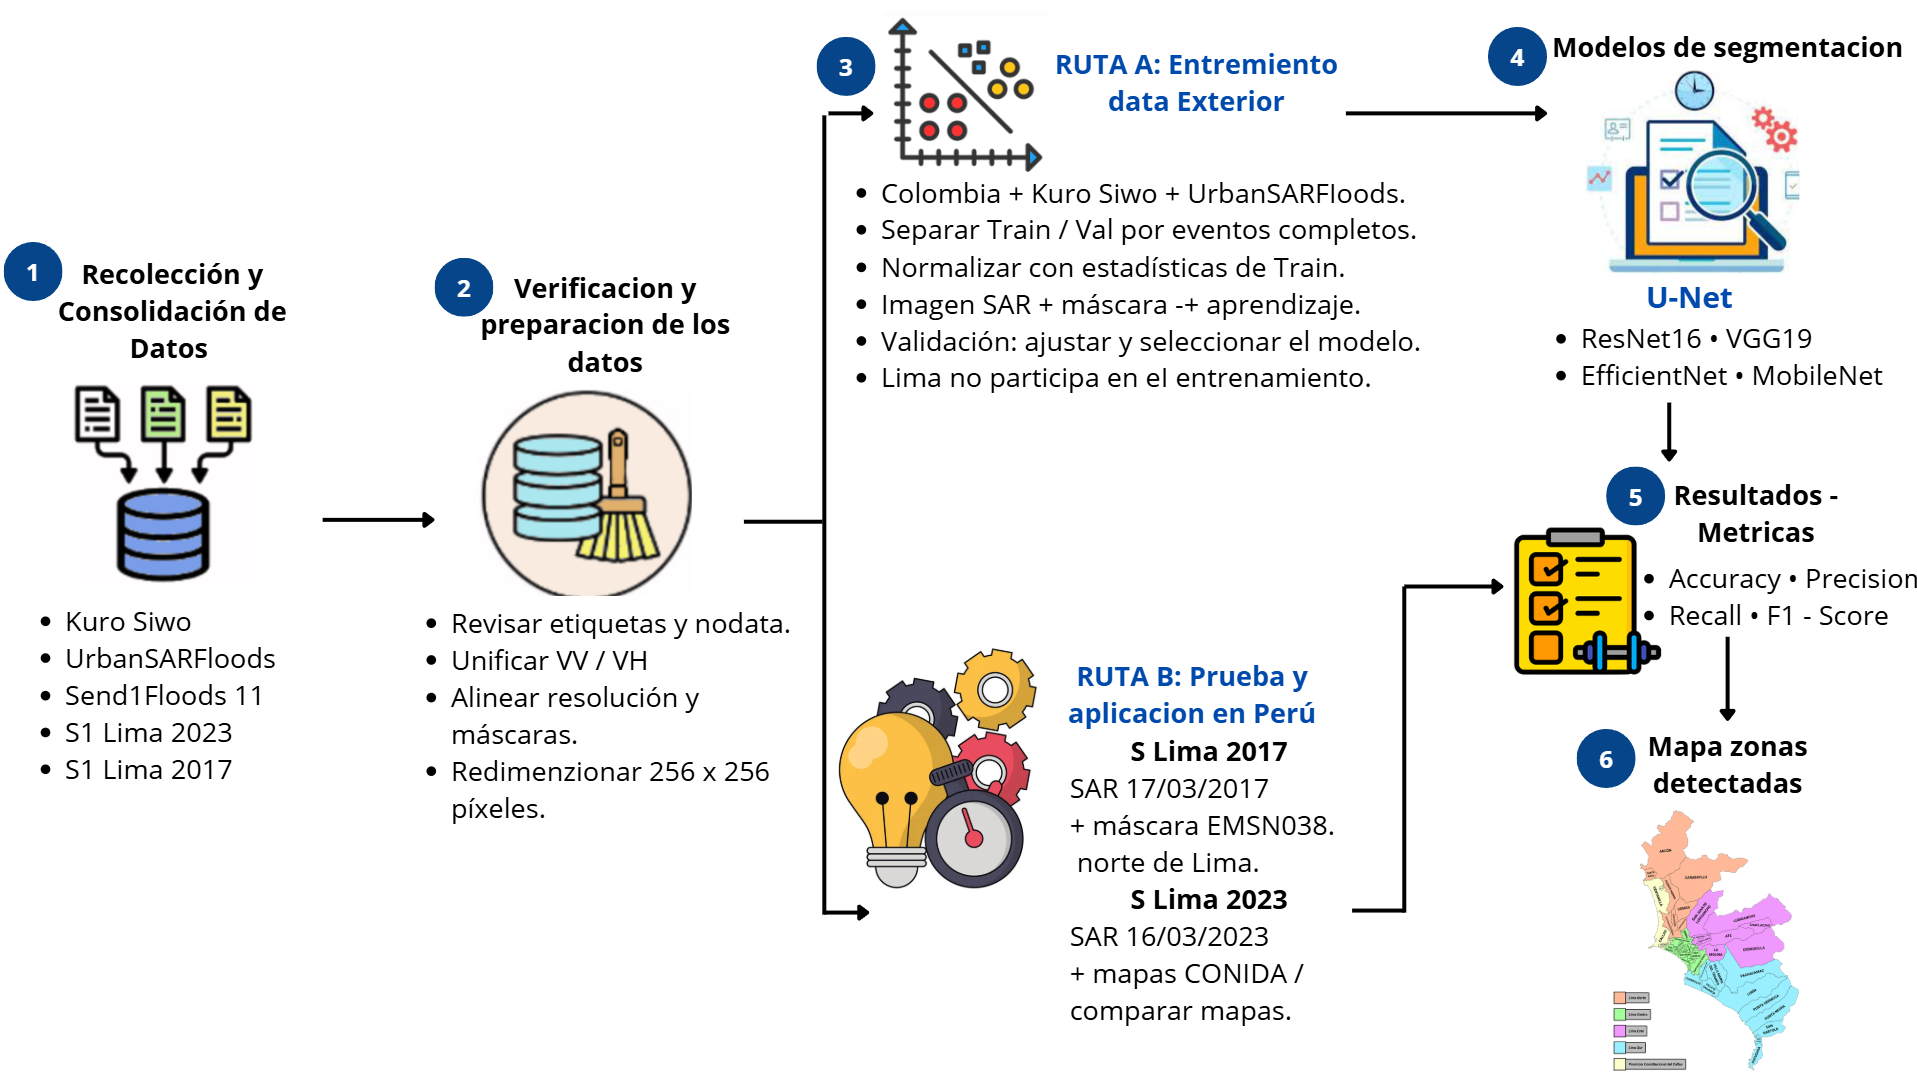
\includegraphics[width=\textwidth]{metodologia_lima_sur.png}
    \caption{Flujo de la metodología propuesta:
    entrenamiento y validación con datasets internacionales,
    prueba y aplicación con datos peruanos, evaluación
    y generación de mapas de zonas detectadas.
    Elaboración propia.}
    \label{fig:metodologia}
\end{figure*}

% ------------------------------------------------------------
\subsection{Conjuntos de datos y recolección}
\label{subsec:datos}

Se consolidarán nueve fuentes de información según su
función experimental: tres datasets internacionales para
entrenamiento y validación, imágenes Sentinel-1 de Lima
de 2017 y 2023, dos fuentes cartográficas de referencia
y dos fuentes de apoyo. Los archivos se organizarán
por dataset, evento, fecha y función dentro del proyecto.

Según el inventario elaborado por el grupo, los datos
disponibles ocupan 84.8~GB. Las cantidades de la
Tabla~\ref{tab:datasets} corresponden a los archivos
reunidos para el proyecto, no al tamaño total de los
datasets publicados ni a la muestra definitiva de
entrenamiento. El inventario reporta una revisión de
formatos mediante las librerías \textit{rasterio}
y \textit{pyogrio}.

Debido al volumen de los datos y a los recursos
computacionales disponibles, no se utilizará
la totalidad de los parches de cada dataset
internacional. Se seleccionarán subconjuntos
para el entrenamiento y la validación.
La Tabla~\ref{tab:datasets} presenta el inventario
disponible; las cantidades efectivamente utilizadas
se documentarán una vez definido el muestreo.

\begin{table*}[!t]
\centering
\caption{Fuentes disponibles y función en la metodología}
\label{tab:datasets}
\footnotesize
\renewcommand{\arraystretch}{1.2}
\setlength{\tabcolsep}{3pt}
\begin{tabular}{
p{0.15\textwidth}
p{0.22\textwidth}
p{0.27\textwidth}
p{0.22\textwidth}
p{0.08\textwidth}
}
\hline
\textbf{Fuente} &
\textbf{Contenido disponible} &
\textbf{Formato reportado} &
\textbf{Función experimental} &
\textbf{Tamaño} \\
\hline

Sen1Floods11 Colombia &
534 parches con etiqueta débil &
VV/VH en dB; $512\times512$;
aprox. 10~m; EPSG:4326 &
Ruta A: entrenamiento &
0.9~GB \\

Kuro Siwo, bloque 00 &
7\,103 parches etiquetados de cinco eventos &
VV/VH en escala lineal; $224\times224$;
10~m; EPSG:3857 &
Ruta A: entrenamiento y validación &
-- \\

UrbanSARFloods &
6\,471 pares de imagen y máscara de 15 eventos &
Ocho bandas; $512\times512$;
aprox. 20~m; EPSG:4326 &
Ruta A: entrenamiento y validación &
-- \\

Sentinel-1 Lima 2017 &
Cuatro escenas Sentinel-1B GRD &
Escenas sin procesar;
polarizaciones según la
Tabla~\ref{tab:escenas2017} &
Ruta B: prueba cuantitativa &
3.1~GB \\

Copernicus EMSN038 &
36 capas; 13 polígonos de inundación &
Geodatabase ESRI; EPSG:32718 &
Referencia de la prueba de 2017 &
2.3~GB \\

Sentinel-1 Lima 2023 &
Once escenas Sentinel-1A GRD &
VV/VH; órbitas 171, 18 y 69 &
Ruta B: aplicación en Lima Sur &
9.2~GB \\

CONIDA 2023 &
Cuatro mapas de zonas afectadas &
Imágenes sin georreferenciar &
Comparación cualitativa en Lima Sur &
41~MB \\

Sen1Floods11 Bolivia &
15 parches manuales y 224 débiles &
Imágenes SAR y máscaras de referencia &
Comparación adicional con la literatura &
0.4~GB \\

JRC, HAND y DEM &
Ocurrencia de agua, altura sobre
el drenaje y elevación &
Resolución aproximada de 30~m &
Interpretación de los mapas &
291~MB \\

\hline
\end{tabular}
\end{table*}

\subsubsection{Datasets internacionales}

\textbf{Sen1Floods11, Colombia.}
Se utilizarán 534 parches de la partición
\textit{WeaklyLabeled} del evento de Colombia
\cite{bonafilia2020sen1floods11}.
Las imágenes contienen las polarizaciones VV y VH
en decibelios. Las máscaras emplean los valores
$-1$ para píxeles sin información, 0 para ausencia
de agua y 1 para presencia de agua. Sus etiquetas
se generaron mediante Otsu sobre imágenes
Sentinel-1 y se considerarán etiquetas débiles.

\textbf{Kuro Siwo, bloque 00.}
El inventario comprende 7\,103 parches etiquetados:
5\,001 de Harvey, 2\,051 de Madagascar,
32 del lago Chad y 19 de Yibuti
\cite{bountos2024kurosiwo}.
Los cinco parches adicionales sin etiqueta
se excluirán. Cada muestra dispone de imágenes
VV/VH, referencias temporales y máscaras con
tres clases: sin agua, agua permanente e inundación.
Las teselas tienen $224\times224$ píxeles a 10~m.
La intensidad está en escala lineal y deberá
convertirse a decibelios.

\textbf{UrbanSARFloods.}
Se utilizarán 6\,471 pares de imagen y máscara
de 15 eventos: 4\,770 de la carpeta sin inundación,
1\,011 de inundación abierta y 690 de inundación
urbana \cite{zhao2024urbansarfloods}.
Las imágenes contienen ocho bandas de intensidad
y coherencia, con resolución aproximada de 20~m.
Para la configuración inicial se seleccionarán
las bandas de intensidad VV y VH durante el evento.
El orden propuesto, bandas 8 y 7 respectivamente,
se confirmará con la documentación antes del
entrenamiento. Las máscaras distinguen áreas
no inundadas, inundación abierta e inundación urbana.

\subsubsection{Imágenes y referencias de Lima}

\textbf{Sentinel-1 Lima 2017.}
Se dispone de cuatro escenas GRD, descritas en
la Tabla~\ref{tab:escenas2017}. Para la prueba
cuantitativa se utilizará la imagen del
17 de marzo de 2017 de la órbita 171 descendente.
La escena del 5 de marzo se conservará como
referencia previa. Las escenas de la órbita 18
contienen únicamente VV y no son compatibles
con la entrada inicial de dos canales.

\begin{table}[!t]
\centering
\caption{Escenas Sentinel-1B disponibles de Lima 2017}
\label{tab:escenas2017}
\footnotesize
\renewcommand{\arraystretch}{1.2}
\setlength{\tabcolsep}{3pt}
\begin{tabular}{cccc}
\hline
\textbf{Fecha} &
\textbf{Momento} &
\textbf{Pasada / órbita} &
\textbf{Pol.} \\
\hline
05/03/2017 & Antes   & Desc. / 171 & VV+VH \\
17/03/2017 & Durante & Desc. / 171 & VV+VH \\
06/03/2017 & Antes   & Asc. / 18   & VV \\
18/03/2017 & Durante & Asc. / 18   & VV \\
\hline
\end{tabular}
\end{table}

\textbf{Copernicus EMSN038.}
La referencia cartográfica de 2017 cubre sectores
del norte de Lima, asociados a los ríos Rímac
y Chillón. Se dispone de una geodatabase de
36 capas en EPSG:32718, un informe y mapas.
Las capas \textit{Potential\_Maximum\_flood}
y \textit{Riverbank} contienen 13 y 11 polígonos,
respectivamente. Se rasterizarán para construir
la referencia binaria. La intersección de
\textit{EMSN038\_AOI} con las seis huellas
de \textit{Footprints} delimitará el área evaluable.

\textbf{Sentinel-1 Lima 2023.}
Se dispone de once escenas GRD con VV y VH,
adquiridas entre el 20 de febrero y el
29 de marzo de 2023. Para la aplicación se propone
la imagen del 16 de marzo de la órbita 171
descendente. La escena del 4 de marzo se
conservará como referencia previa. También
se dispone del par del 5 y 17 de marzo de
la órbita 18 ascendente.

\textbf{Mapas CONIDA 2023.}
Se dispone de cuatro mapas: Punta Hermosa,
obtenido con TerraSAR-X el 15 de marzo;
Pachacámac, con PeruSAT-1 el 17 de marzo
y WorldView-3 el 18 de marzo; y
Chilca--Pucusana, con PeruSAT-1 el 22 de marzo.
Las imágenes se georreferenciarán en QGIS
mediante puntos de control y las zonas de
interés se digitalizarán para la comparación
cualitativa.

\subsubsection{Fuentes de apoyo}

El evento de Bolivia de Sen1Floods11 se reservará
para una comparación adicional con la literatura
\cite{bonafilia2020sen1floods11}.
Se dispone de 15 parches con etiqueta manual
y 224 con etiqueta débil. Ninguno se utilizará
para entrenar ni seleccionar el modelo.

Las capas JRC Global Surface Water, HAND y
Copernicus DEM GLO-30 se utilizarán como apoyo
para interpretar las detecciones, no como
canales de entrada. Se reproyectarán a la
grilla de las escenas de Lima. La ocurrencia
histórica de agua ayudará a identificar
posibles cuerpos permanentes, mientras que
HAND y pendiente permitirán examinar la
plausibilidad de las detecciones.

% ------------------------------------------------------------
\subsection{Verificación y preparación de los datos}
\label{subsec:preparacion}

Se revisarán las bandas, unidades de retrodispersión,
resolución espacial, coordenadas y valores de las
etiquetas de cada fuente. Los píxeles sin información
se registrarán en una máscara de validez para
excluirlos de la pérdida y de las métricas.

Se unificará el orden de los canales VV y VH.
Los datos en potencia lineal se convertirán
mediante $10\log_{10}(x)$ sobre valores positivos
y válidos. Se propone limitar la entrada al rango
$[-30,5]$~dB.

Las escenas GRD de Lima se procesarán en SNAP
mediante aplicación de órbita, calibración
radiométrica a $\sigma^{0}$, filtrado de
\textit{speckle} con Refined Lee y corrección
de terreno. Se convertirán a decibelios
y se organizarán en una grilla de 10~m
en EPSG:32718.

Las imágenes y máscaras se alinearán espacialmente.
Las máscaras se remuestrearán mediante vecino
más cercano para preservar sus clases.
El remuestreo de UrbanSARFloods de 20 a 10~m
permitirá armonizar la grilla, pero no recuperará
detalle espacial de la imagen original.

Se generarán parches de $256\times256$ píxeles
mediante recorte o relleno. En Kuro Siwo,
las teselas de $224\times224$ se completarán
con relleno, que quedará excluido de la pérdida
y de la evaluación. La entrada inicial tendrá
dimensiones $256\times256\times2$, correspondientes
a VV y VH durante el evento.

Para la configuración binaria se agruparán
las clases de agua permanente e inundación
como clase positiva, cuando estén diferenciadas
en la fuente. Se conservará un registro de
la procedencia y naturaleza de las etiquetas.
Esta configuración no distinguirá por sí sola
el agua permanente de la inundación nueva.

% ------------------------------------------------------------
\subsection{Partición experimental}
\label{subsec:particion}

La separación se realizará por eventos completos,
antes de seleccionar muestras y calcular
las estadísticas de normalización. Se evitará
que parches de un mismo evento aparezcan
en entrenamiento y validación.

La Tabla~\ref{tab:particion} presenta la distribución
propuesta. Harvey aparece tanto en Kuro Siwo como
en UrbanSARFloods y se asignará íntegramente
al entrenamiento. Las muestras de Madagascar
de la misma temporada se mantendrán juntas
en validación. Los cuatro eventos australianos
de UrbanSARFloods también se reservarán
para validación.

Se priorizará la independencia entre eventos
sobre una proporción fija de 80/20. No se
utilizará directamente la partición oficial
de UrbanSARFloods si distribuye parches
del mismo evento entre ambos conjuntos.

\begin{table}[!t]
\centering
\caption{Partición propuesta por eventos completos}
\label{tab:particion}
\footnotesize
\renewcommand{\arraystretch}{1.2}
\begin{tabular}{
@{}p{0.23\columnwidth}
p{0.68\columnwidth}@{}
}
\hline
\textbf{Conjunto} & \textbf{Contenido} \\
\hline

Entrenamiento &
Sen1Floods11 Colombia; Kuro Siwo:
Harvey, lago Chad y Yibuti;
UrbanSARFloods: once eventos no australianos,
incluidos Houston 2016 y 2017. \\

Validación &
Kuro Siwo: Madagascar, 2\,051 parches;
UrbanSARFloods: Port Macquarie 2021,
Sídney 2021, Sídney 2022 y Coraki 2022. \\

Prueba &
Lima, 17/03/2017, con referencia EMSN038. \\

Aplicación &
Lima Sur, 16/03/2023, comparada con CONIDA. \\

Comparación adicional &
Sen1Floods11 Bolivia:
15 parches con etiqueta manual. \\

\hline
\end{tabular}
\end{table}

Después de separar los eventos entre entrenamiento
y validación, se seleccionará una muestra de
parches dentro de cada partición. El muestreo
considerará la representación de los eventos
y de los parches con y sin presencia de agua,
para reducir el predominio de las fuentes
con mayor cantidad de muestras.

Se documentarán el criterio de selección,
la cantidad de parches utilizada por dataset
y evento, y la distribución de las clases.
Se empleará la semilla aleatoria 42 para
permitir la reproducción del muestreo.

La media y desviación estándar por canal
se calcularán únicamente con los píxeles
válidos de la muestra de entrenamiento.
Estas estadísticas se reutilizarán en
validación, prueba y aplicación.
Los datos peruanos permanecerán reservados
para prueba y aplicación.

% ------------------------------------------------------------
\subsection{Modelos de segmentación y entrenamiento}
\label{subsec:modelos}

Se utilizará U-Net como arquitectura de segmentación,
con un codificador para extraer características
y un decodificador para recuperar la distribución
espacial mediante conexiones de salto.
Se considerará comparar codificadores de
las familias ResNet, EfficientNet, VGG19
y MobileNet. Las variantes específicas
se confirmarán antes de los experimentos.

Estas redes se integrarán como codificadores
de U-Net y no como clasificadores independientes
de imágenes. La salida será una probabilidad
por píxel de pertenecer a la clase positiva.

Los modelos se entrenarán exclusivamente con
los datos internacionales de la ruta A.
Se propone combinar entropía cruzada binaria
y pérdida Dice sobre los píxeles válidos.
Como configuración inicial se utilizará
Adam con tasa de aprendizaje de $10^{-4}$,
un máximo de 50 épocas y parada temprana
según la IoU de validación, con paciencia
de cinco épocas.

Se considerarán lotes de 8 a 16 parches
y aumentos mediante rotaciones de $90^{\circ}$
y reflexiones. Las transformaciones se
aplicarán conjuntamente a la imagen,
su máscara y la máscara de validez.

La comparación y selección de configuraciones
se realizará con la validación internacional.
Se propone un umbral inicial de 0.5 para
obtener máscaras binarias. Cualquier ajuste
de este umbral se realizará con validación
y quedará fijado antes de consultar la prueba.

Se conservarán los parámetros, las estadísticas
de normalización y las curvas de aprendizaje.
El modelo seleccionado se aplicará a Lima
sin reentrenamiento ni ajuste fino local.

% ------------------------------------------------------------
\subsection{Prueba y aplicación con datos peruanos}
\label{subsec:evaluacion}

La ruta B utilizará las imágenes peruanas para
examinar el desempeño del modelo fuera del
dominio de entrenamiento. Se distinguirá
la prueba cuantitativa de 2017 de la aplicación
cualitativa en Lima Sur 2023.

\subsubsection{Evaluación cuantitativa de 2017}

Las predicciones sobre la imagen del
17 de marzo de 2017 se compararán con
la referencia rasterizada de EMSN038.
La evaluación se limitará al área definida
por sus coberturas y excluirá los píxeles
sin información.

Se reportarán IoU, precisión, \textit{recall}
y F1  de la clase positiva.
La exactitud global se considerará complementaria
por el posible predominio de píxeles sin agua.

Para los conteos binarios agregados:

\begin{equation}
\mathrm{IoU} =
\frac{TP}{TP+FP+FN},
\end{equation}

\begin{equation}
\mathrm{Precision} =
\frac{TP}{TP+FP},
\end{equation}

\begin{equation}
\mathrm{Recall} =
\frac{TP}{TP+FN},
\end{equation}

\begin{equation}
\mathrm{F1} =
\frac{2TP}{2TP+FP+FN},
\end{equation}

donde $TP$, $FP$ y $FN$ representan verdaderos
positivos, falsos positivos y falsos negativos.
Con la misma agregación binaria, Dice y F1
son equivalentes.

EMSN038 cubre sectores del norte de Lima.
Por tanto, esta prueba permitirá evaluar
la transferencia a un evento peruano,
pero no demostrará directamente el desempeño
cuantitativo en Lima Sur. También se considerará
el desfase entre el radar del 17 de marzo
y las referencias ópticas del 18 y 21 de marzo.

\subsubsection{Aplicación en Lima Sur 2023}

Se aplicará el modelo a la imagen del
16 de marzo de 2023 y se compararán sus
predicciones con los mapas CONIDA
georreferenciados. Se examinará la coincidencia
espacial entre detecciones y zonas cartografiadas,
considerando las diferencias de fecha,
sensor y cobertura.

Esta comparación será cualitativa mientras
no se disponga de máscaras independientes,
espacial y temporalmente compatibles.
Los datos peruanos no se utilizarán
para seleccionar parámetros ni actualizar
los pesos de la red.

\subsubsection{Comparación adicional}

Opcionalmente, se evaluará el modelo con
los 15 parches manuales de Bolivia.
La comparación con resultados publicados
deberá considerar la definición de clases,
los píxeles válidos y el protocolo de evaluación
para evitar atribuir equivalencia a experimentos
con condiciones distintas.

% ------------------------------------------------------------
\subsection{Generación de mapas y limitaciones}
\label{subsec:mapas}

Las predicciones de los parches se reconstruirán
en la grilla geográfica de las escenas.
Se conservarán las coordenadas y las máscaras
de validez para generar mapas de las zonas
detectadas y examinar errores de omisión
y comisión.

Las capas JRC, HAND y DEM apoyarán
la interpretación de los resultados.
La ocurrencia histórica de agua superior
al 80\% se considerará un indicador de
posible agua permanente, no una referencia
infalible. Los valores altos de HAND
y las pendientes mayores a $15^{\circ}$
se utilizarán como indicios para revisar
detecciones, sin asumir que descartan
todo anegamiento urbano.

La interpretación considerará cinco
limitaciones principales: las etiquetas
débiles de Colombia; la resolución original
de 20~m de UrbanSARFloods; la cobertura
externa y el desfase temporal de EMSN038;
las restricciones de georreferenciación
y comparabilidad de CONIDA; y el predominio
de Harvey en el subconjunto de Kuro Siwo.

Además, la clase positiva inicial agrupa
agua permanente e inundación. Por ello,
los mapas se presentarán como detecciones
de presencia de agua durante el evento,
sin afirmar que todos los píxeles positivos
corresponden a inundación nueva.

Se distinguirán explícitamente los resultados
cuantitativos de la prueba externa de 2017
de los resultados cualitativos de aplicación
en Lima Sur 2023.

% ============================================================
% (Secciones siguientes: fuera del alcance del Avance 1 según la
% actividad, pero se dejan los encabezados para que el documento
% final no requiera reestructurar todo desde cero)
% ============================================================

% \section{Metodología Propuesta}
% \label{sec:metodologia}
% % Se completa en una entrega posterior: describir el pipeline de
% % 6 fases (adquisición, preprocesamiento, etiquetado automático,
% % preparación de dataset, entrenamiento, evaluación).

% \section{Experimentos y Resultados}
% \label{sec:experimentos}

% \section{Conclusiones}
% \label{sec:conclusiones}

% ============================================================
% REFERENCIAS
% Usando BibTeX. El archivo .bib correspondiente se entrega aparte
% (referencias.bib) con las 4 entradas ya completas y listas.
% ============================================================
\bibliographystyle{IEEEtran}
\bibliography{referencias}

\end{document}